%!TEX root = ../thesis.tex
%*******************************************************************************
%*********************************** Fifth Chapter *****************************
%*******************************************************************************

\chapter{Smoothing}
\ifpdf
    \graphicspath{{Chapter5/Figs/Raster/}{Chapter5/Figs/PDF/}{Chapter5/Figs/}}
\else
    \graphicspath{{Chapter5/Figs/Vector/}{Chapter5/Figs/}}
\fi

Lattice definitions of topological objects are plagued by random fluctuations originating from the Monte-Carlo generation of lattice configuration and as a result they can often give inaccurate or nonsensical results. Hence, when considering the behaviour of topological objects on the lattice, it has been proven to be necessary to remove high frequency fluctuations in the gauge fields~\cite{Bonnet:2000dc}. Furthermore, when investigating the long distance behaviour of the lattice it is also beneficial to filter off the short distance fluctuations to better reveal the physics in the region of interest~\cite{Moran:2008ra}. For example, it has previously been shown that smoothing is necessary to obtain agreement between the untouched and vortex only string tension, mass function and instanton content~\cite{Trewartha:2015ida,Trewartha:2015nna,Trewartha:2017ive}. The process of removing these fluctuations is known as smoothing, which in turn falls into two sub-categories: cooling and smearing.\\

The purpose of both these methods is similar, however, the algorithms used to implement them differ greatly. Cooling assesses each link, replacing the existing link with one that locally minimises some choice of action (see e.g. the Wilson action in Eq.~\ref{eq:WilsonAction}). Smearing does not depend on the choice of action, and instead replaces each link with a weighted average of its nearest neighbours. Once every link in the lattice has been updated, the configuration is said to have had one sweep of smoothing applied. The process can then be repeated to an arbitrary number of sweeps.  Due to the differences in the routines, it is important to compare the results from both to observe how they each perform and quantitatively observe how the alter the measured quantities.


%Motivated by these results, we now investigate the effect of both $\mathcal{O}(a^4)$-improved cooling~\cite{BilsonThompson:2003zi} and over-improved stoutlink smearing~\cite{Moran:2008ra}. Following the results of Ref.~\cite{Moran:2008ra}, the over-improved smearing parameters are $\rho=0.06$ and $\epsilon=0.25$ to best preserve the size of instantons on the lattice. To accomplish a similar preservation of topological objects under cooling, we used the three-loop improved algorithm as described in Ref.~\cite{BilsonThompson:2003zi}.\\
\section{Smoothing Methods}
\subsection{Cooling}
Cooling is the original method devised for smoothing lattice gauge fields, first utilised in the analysis of the topological susceptibility of simplified lattice models~\cite{Berg:1981nw}. It was shown early on that the process of cooling can be used to distinguish between 'genuine' topological charge representative of classical minima of the action, and background Monte-Carlo topological charge brought about by random fluctuations created during the generation of the lattice configuration. Under cooling, the former is preserved whilst the latter is annihilated. The process of cooling according to the simplest Wilson action is based on the method outlined by Cabibbo and Marinari~\cite{Cabibbo:1982zn,Creutz:1980zw}, and is performed as follows:\\

We first consider the Wilson action associated with a single link $U_\mu$, 
\begin{equation}
S(U_\mu) = 3 - \operatorname{Re}\Tr (U_\mu \bar{U})\, ,
\label{eq:WilsonActionCool}
\end{equation}
which is a different, but completely equivalent, form of Eq.~\ref{eq:WilsonAction}. $\bar{U}$ is defined as the sum of the `staples' associated with $U_\mu$.  A staple is defined as the product of all the link variables around a chosen loop, except for the link being cooled. For example, the $1\times 1$ plaquette staple associated with $U_\mu$ is
%
\begin{equation}
\tilde { U }^{1\times 1} _ { \mu }(x) = U _ { \nu } ( x + \hat { \mu } ) U _ { \mu } ^ { \dagger } ( x + \hat { \nu } ) U _ { \nu } ^ { \dagger } ( x )\, .
\end{equation}
%
Graphically, this can be seen as in Fig.~\ref{fig:Staple}.
\begin{figure}[h!]
\centering
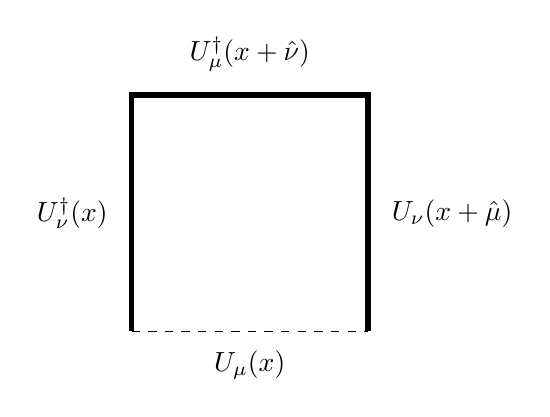
\begin{tikzpicture}
\draw[line width = 2pt] (0,-3) -- (0,0)node[midway, label=right:{$U_\nu(x+\hat{\mu})$}]{} -- (-3,0)node[midway, label=above:{$U_\mu^\dag(x+\hat{\nu})$}]{} -- (-3,-3)node[midway, label=left:{$U_\nu^\dag(x)$}]{};
\draw[dashed] (-3,-3) -- (0,-3)node[midway, label=below:{$U_\mu(x)$}]{};
%\draw plot[mark=*,mark size = 3pt,mark options={color=red}] coordinates {(-3,-3)(0,-3)(0,0)(-3,0)};
\end{tikzpicture}
\caption{\label{fig:Staple} An example $1\times 1$ staple, with the dashed link indicating the link the staple is relative to. The origin of the name staple is apparent from the shape of the 3 solid links.}
\end{figure}
Larger staples are defined similarly; for example a $2\times 2$ staple corresponds to the product of seven of the eight links in the $2\times 2$ square, with $U_\mu(x)$ omitted. For the Wilson action, the six unique $1\times 1$ staples are the only ones required. Once all relevant staples are calculated, they are summed to obtain
%
\begin{equation}
\bar{U} = \sum_{\alpha = 1} ^ 6 \tilde{U}_\alpha\, ,
\label{eq:Staples}
\end{equation}
where $\alpha$ enumerates the staples, not the Lorentz index.\\
%

The objective of cooling is to select a new $SU(3)$ matrix to replace $U_\mu$ with some $U_\mu^\prime$ that minimises Eq.~\ref{eq:WilsonActionCool}, or equivalently, maximises
\begin{equation}
\operatorname{Re} \Tr (U_\mu^\prime \, \bar{U})\, .
\end{equation}
Naively, it would seem that $U_\mu^\prime = \bar{U}^{-1}$ would be the ideal choice. However, $\bar{U}$ is the sum of $SU(3)$ matrices, and $SU(3)$ is only closed under multiplication, not addition. Hence, $\bar{U}$, and by extension $\bar{U}^{-1}$, are not necessarily in $SU(3)$, making $\bar{U}^{-1}$ and invalid substitute for $U_\mu$. However, any $SU(2)$ element can be written in the form $U = a _ { 0 } I + i \vec { a } \cdot \vec { \sigma }$, where $\vec{\sigma}$ are the Pauli matrices and $a\in\mathbb{R}$  satisfies $a^2=1$. Hence, a sum of $SU(2)$ elements is proportional to another $SU(2)$ element. We can exploit this fact to construct an new $SU(3)$ element from three $SU(2)$ subgroups. To this end, we wish to find a $U^\prime$ of the form
%
\begin{equation}
U^\prime_\mu = a_3\,a_2\,a_1\,U_\mu\, ,
\label{eq:UPrime}
\end{equation}
%
where the $a_i$ are each in different a $3\times 3$ representation of $SU(2)$. We define the following three functions to take some $V\in SU(3)\rightarrow F_i(V)\in SU(2)$
%
\begin{align*}
F_1(V) &=\frac{1}{k_1} \begin{pmatrix}
\frac{1}{2}\left(V_{11} + V_{22}^*\right) & \frac{1}{2}\left(V_{12} - V_{21}^*\right) & 0\\
\frac{1}{2}\left(V_{21} - V_{12}^*\right) & \frac{1}{2}\left(V_{11}^* + V_{22}\right) & 0\\
0 & 0 & 1
\end{pmatrix}\\
F_2(V) &=\frac{1}{k_2} \begin{pmatrix}
\frac{1}{2}\left(V_{22} + V_{33}^*\right) & 0 &\frac{1}{2}\left(V_{23} - V_{32}^*\right)\\
0 & 1 & 0\\
\frac{1}{2}\left(V_{32} - V_{23}^*\right) & 0 & \frac{1}{2}\left(V_{22}^* + V_{33}\right)
\end{pmatrix}\\[10pt]
F_3(V) &=\frac{1}{k_3} \begin{pmatrix}
1 & 0 & 0\\
0 & \frac{1}{2}\left(V_{11} + V_{33}^*\right) & \frac{1}{2}\left(V_{13} - V_{31}^*\right)\\
0 & \frac{1}{2}\left(V_{31} - V_{13}^*\right) & \frac{1}{2}\left(V_{11}^* + V_{33}\right)
\end{pmatrix}\, ,
\end{align*}
%
where $k_i^2 = \det(k_i\, F_i(V))$ fixes the determinant such that $\det(F_i(V))=1$.
We now wish to find a suitable $V$ to define our $a_i$'s. Consider the first case, $U^{(1)}_\mu = a_1\,U_\mu$, and let $a_1 = F_1(U_\mu\,\bar{U})^\dagger$. It is worth stating explicitly that it is this step where the fact that a sum of $SU(2)$ matrices is proportional to an $SU(2)$ matrix is utilised. Despite the fact that $U_\mu\,\bar{U} \notin SU(3)$, $U_\mu \, \tilde{U}_\alpha\in SU(3)$, which implies that $F_i(U_\mu\, \tilde{U}_\alpha)\in SU(2)$. Then we have
%
\begin{align}
\sum_{\alpha=1}^6 k_{i,\,\alpha} \, F_i(U_\mu\, \tilde{U}_\alpha) &= k_i F_i(U_\mu \bar{U}) \label{eq:SU2Sum}\\
\implies F_i(U_\mu \bar{U}) &= \frac{1}{k_i}\sum_{\alpha=1}^6 k_{i,\,\alpha} \, F_i(U_\mu\, \tilde{U}_\alpha)\in SU(2)\, ,\nonumber
\end{align}
%
where we have made use of the linearity of $k_i\,F_i$ to obtain Eq.~\ref{eq:SU2Sum}. With this definition of $a_1$, the functional we are seeking to maximise evaluates to
%
\begin{equation}
\operatorname{Re} \Tr (F_1(U_\mu\,\bar{U})^\dagger \, U_\mu \, \bar{U}) = 2 + \Re(U_\mu\, \bar{U})_{33}\, .
\label{eq:MaximisedCooling}
\end{equation}
%
The proof of this is given in Appendix \ref{app:CoolingMaximise}. By the matrix structure of $F_1(V)$ it is apparent that $\Re(U_\mu\, \bar{U})_{33}$ is invariant under pre-multiplication by $a_1$, so it is clear that Eq.~\ref{eq:MaximisedCooling} represents the maximum attainable value for this form of $U^{(1)}_\mu$. Similarly, we let $a_2=F_2(U_\mu\,\bar{U})^\dagger$ and $a_3=F_3(U_\mu\,\bar{U})^\dagger$ to obtain the final value of $U^\prime_\mu$ according to Eq.~\ref{eq:UPrime}. The above procedure is repeated over all three $SU(2)$ subgroups 12 times per lattice link to effectively minimise the local action. One sweep of cooling then constitutes applying this procedure to every link on the lattice.\\

As detailed in Ref.~\cite{Bonnet:2000dc}, this process can be thought of as locally minimising the Wilson action of the three $SU(2)$ subgroups, which collectively minimises the Wilson action of the full $SU(3)$ link. It is then simple to extend this procedure to different actions by expanding the size and shape of the staples considered in the construction of $\bar{U}$. As the only quantities utilised in the cooling procedure are gauge invariant, cooling can be performed in any gauge to arrive at the same cooled configuration. Cooling also maintains the Boltzmann distribution of the lattice links~\cite{Cabibbo:1982zn}, indicating that the new links can be considered a thermalised distribution. However, cooling is not a gauge transformation, and as such it represents a deviation from the original physical configuration. We therefore need to be careful when selecting the action used for the cooling routine to ensure that we are not removing the physics that we are interested in. To best study instantons and topological charge on a periodic lattice, it has been shown that a $\mathcal{O}(a^4)$ three-loop  improved action is most suitable~\cite{BilsonThompson:2002jk}. This choice of action combines both computational efficiency with an effective stabilisation of instantons and an accurate preservation of the topological charge under repeated cooling sweeps. This action is dubbed a `three-loop' action as it consists of a linear combination of $1\times 1$, $2\times 2$ and $3\times 3$ Wilson loops.

\subsection{Over-Improved Smearing}
Despite the accurate results obtained from cooled lattice configurations, cooling presents certain computational inefficiencies. Given that the staples, $\bar{U}_\alpha$ must remain constant while updating a given link $U_\mu$, there are limitations to how  parallelised the algorithm can be, especially for larger combinations of loops such as those used in the chosen three-loop improved action. To avoid these issues, a different type of smoothing was developed, known as `smearing'. Rather than locally minimising the action by direct substitution of each link, the initial APE smearing~\cite{Albanese:1987ds, Falcioni:1984ei} routine replaces each link with a weighted average of its nearest neighbours, according to
%
\begin{equation}
U^\prime = (1-\alpha)\,U_\mu + \frac{\alpha}{6}\,\bar{U}^\dagger\, ,
\end{equation}
%
where $\bar{U}$ is the sum of the staples given in Eq.~\ref{eq:Staples} and $\alpha$ is some weighting parameter. However, as stated in the previous section, a linear combination of $SU(3)$ matrices is not necessarily in $SU(3)$, so APE smearing is dependent on a choice of projection into the $SU(3)$ group. To remove the need for this projection step, the method of stout-link smearing was developed~\cite{Morningstar:2003gk}.\\

Much like in the case of cooling, it is easiest to begin by considering smearing in terms of the Wilson action, then extending this to the over-improved case utilised in this research. To begin, we define
%
\begin{equation}
\Sigma_\mu = \rho_\text{sm}\,(U_\mu\,\bar{U})^\dagger\, ,
\end{equation}
%
where $\rho_\text{sm}$ is a smearing constant chosen to remain fixed for all lattice sites. Using this definition we construct
%
\begin{equation}
Q_\mu = \frac{i}{2}\left( \Sigma_\mu^\dagger - \Sigma_\mu \right) - \frac{i}{6}\Tr\left(\Sigma_\mu^\dagger - \Sigma_\mu\right)I\, .
\end{equation}
By construction $Q_\mu$ is Hermitian ($Q_\mu = Q_\mu^\dagger$) and traceless, so it belongs to the $SU(3)$ Lie algebra. It can therefore be exponentiated to obtain an element of $SU(3)$. We then define the new smeared link by
%
\begin{equation}
U_\mu^\prime = \exp(iQ_\mu)\,U_\mu\, .
\end{equation}
%
This definition effectively corresponds to a complex sum of neighbouring link combinations, however it has numerically been demonstrated to give similar results to the previous APE smearing technique, provided that the smearing parameter $\rho$ is selected appropriately~\cite{Morningstar:2003gk}. As in the case of cooling, the choice of staples used to define $\bar{U}$ has significant impact on the behaviour of topological objects under smearing. To this end, work has been done to tune the smearing algorithm so that it preserves instanton-like objects under repeated smearing sweeps, leading to the development of over-improved stoutlink smearing~\cite{Moran:2008ra}.\\

To quantitatively measure the effect of smearing on topological objects, it is common to calculate the instanton action in terms of the instanton radius. The error terms in the instanton action then give an indication of how the instanton radius will change as the action decreases under smearing.
\section{Results from the Gluon Propagator}\label{sec:CoolingGluProp}

\begin{figure}[tb]
\centering
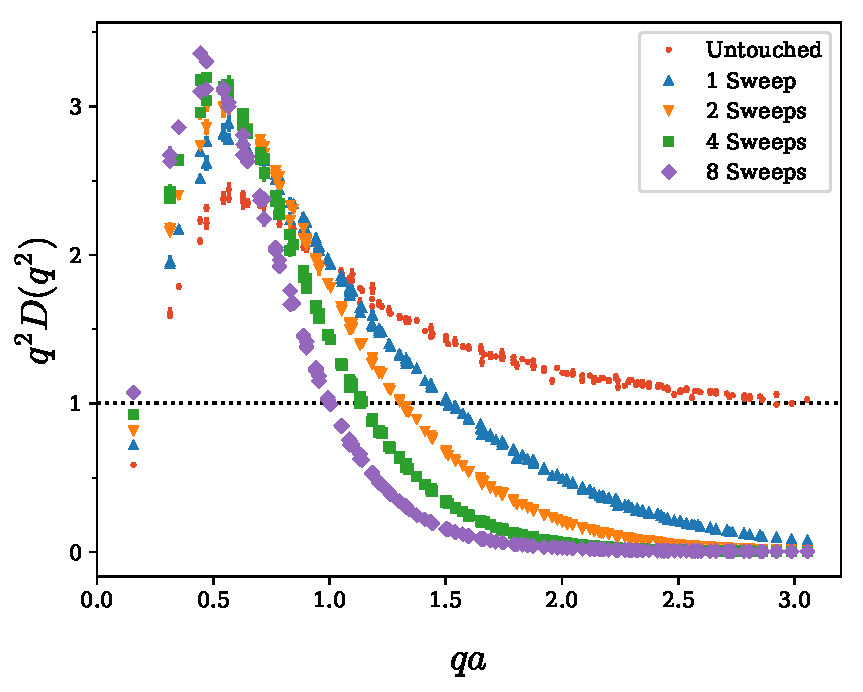
\includegraphics[width=\linewidth]{./ScalarGluComp_q2_1to10sweeps.pdf}
\caption{\label{fig:1to10SweepsCooling}Comparison of the gluon propagator on the untouched configurations after cooling. For clarity we have selected a sample of sweeps between 1 and 8.}
\end{figure}
%

Making use of the smoothing methods defined above, we now wish to compare their effect on the gluon propagator. We first plot the untouched propagator after 0, 1, 2, 4 and 8 sweeps of cooling in Fig.~\ref{fig:1to10SweepsCooling}. In gauge fixing to Landau gauge, each sweep has been preconditioned by the Landau gauge transformation of the prior sweep in descending order (i.e. the transformation for sweep 10 preconditions sweep 9). This preconditioning is done to ensure that the Landau gauge functional is near the same local minima for each cooling sweep. We observe the expected removal of short distance fluctuations that is typical of smoothing, resulting in a suppressed propagator at large $q$. This is complemented by an amplification in the infra-red region which can be attributed to the increase in low momentum modes arising from the smoothing of the gauge fields.\\
%
\begin{figure}[tb]
\centering
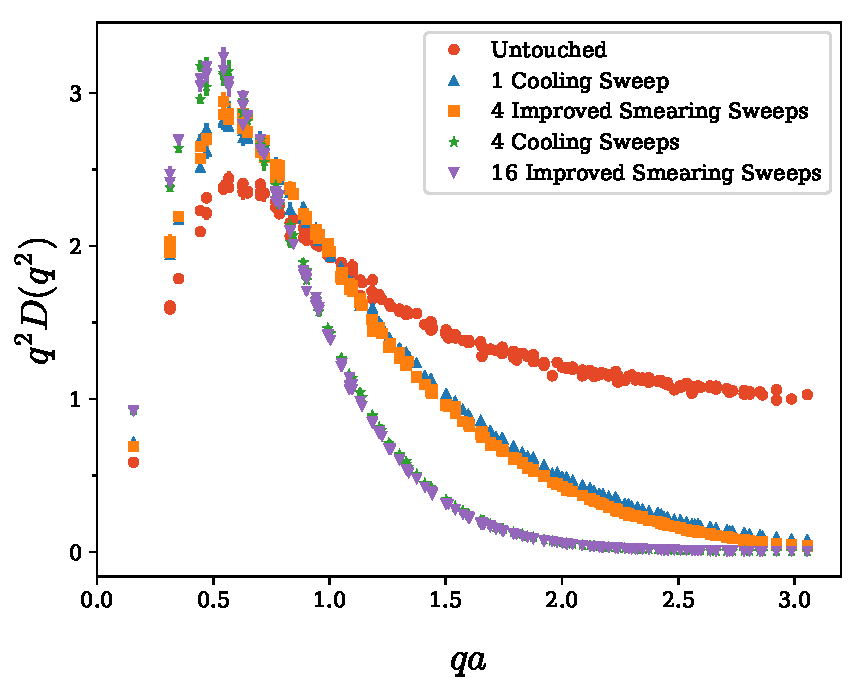
\includegraphics[width=\linewidth]{./ScalarGluComp_q2_SmearCoolComp.pdf}
\caption{\label{fig:SmearCoolComp}The gluon propagator after cooling or improved smearing. We see that the shape of the plot changes minimally between the smoothing routines. However cooling requires fewer sweeps to produce the same effect when compared to smearing.}
\end{figure}
%

To compare the effects of cooling and over-improved smearing, the untouched gluon propagator is plotted in Fig.~\ref{fig:SmearCoolComp} after either over-improved smearing or cooling. By comparing the smeared and cooled propagator we can see that cooling has a more rapid effect, related to the well-known fast removal of action from the lattice. The qualitative shape of the propagator remains the same however, and it can be seen that, for example, 4 smearing sweeps produces a propagator remarkably similar to 1 cooling sweep. More generally, we observe that in regards to the shape of the propagator, $n_{\text{sm}}\approx4\,n_{\text{cool}}$. Following the observation made in Ref.~\cite{Thomas:2014tda} that the number of over-improved stoutlink smearing sweeps is related to the gradient flow time by
%
\begin{equation}
t\approx\rho\,n_{\text{sm}}\, ,
\end{equation}
%
we deduce that the relationship between gradient flow time and cooling is
\begin{equation}
t\approx0.24\,n_{\text{cool}}\,.
\end{equation}\\

It is well understood that smoothing alters the vortex background, and based on previous work~\cite{Cais:2008za,Trewartha:2015ida,DelDebbio:1998luz} we anticipate that the vortices identified on smoothed configurations would differ to those identified on the unsmoothed configurations. We therefore perform vortex identification only on the original configurations, with smoothing then being performed independently on the untouched, vortex-only and vortex-removed configurations. We choose to use cooling as the smoothing algorithm for the results presented in this paper, however it is worth noting that similar results can be obtained with the use of over-improved smearing. 

